\documentclass[titlepage,landscape]{seminar}
\usepackage{url}
\usepackage{graphicx}
\usepackage[pdftex]{color}
\usepackage{hyperref}
\usepackage{epstopdf}
\usepackage{slides}

\newcommand{\frack}{\frac{1}{k}}

\begin{document}

\myslide{
\heading{Nei's $G_{ST}$}
\begin{eqnarray*}
H_{i} &=& 1 - {1 \over N} \sum_{k=1}^{N} \sum_{i=1}^{m} {X_{kii}} \\
H_{s} &=& {\tilde n \over {\tilde n - 1}}
         \left[1 - \sum_{i=1}^{m} {\bar {\hat x_{i}^{2}}}
         - {H_{I} \over {2 \tilde n}}\right] \\
H_{t} &=& 1 - \sum_{i=1}^{m} {\bar x_{i}^{2}} + {H_{S} \over {\tilde n}}
         - {H_{I} \over {2 \tilde n N}}
\end{eqnarray*}
}

\myslide{
\begin{itemize}

\item {\it Statistical sampling} - Repeated samples from the same
  population differ from one another. For example, the sample
  frequency of an allele, $\hat p$, will differ from sample to sample
  even if the ``true'' population frequency, $p$, is always the same. 

\item {\it Genetic (or evolutionary) sampling} - We are rarely, if
  ever, interested only in the populations or loci we sampled. We are
  almost always interested in using them as ``representatives'' of all
  populations or loci that could have been sampled. In other words the
  populations and loci we actually studied are best regarded as a
  sample from the set of all comparable populations and loci that
  could have been studied.

\end{itemize}
}

\myslide{
\begin{center}
\resizebox{!}{\textheight}{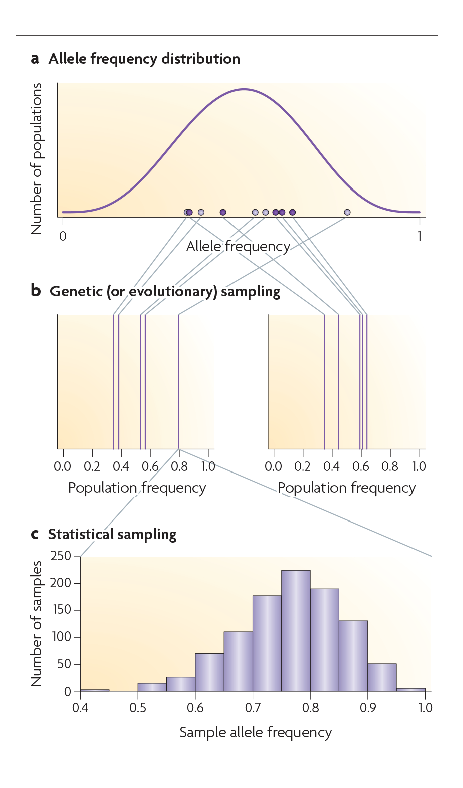
\includegraphics{sampling.eps}}
\end{center}
}

\myslide{
\heading{Weir \& Cockerham's $\theta$}
\begin{itemize}

\item $x_{ijk} = 0,1$ - Indicator of whether allele $A_1$ is present
  in chromosome $i$ of individual $j$ in population $k$

\item Nested analysis of variance on indicator variables (chromosomes,
  within individuals, within populations)

\item Components of variance related to $F_{IS}$, $F_{ST}$, and
  $F_{IT}$

\end{itemize}
}

\myslide{
\heading{Estimates of $F_{ST}$}
\begin{center}
  \begin{tabular}{c|ccc}
\hline\hline
Method & $F_{is}$ & $F_{st}$ & $F_{it}$ \\
\hline
Direct            & 0.1372 & 0.2143 & 0.3221 \\
Nei               & 0.3092 & 0.2395 & 0.4746 \\
Weir \& Cockerham & 0.5398 & 0.0387 & 0.5577 \\
\hline
\end{tabular}
\end{center}
\vfill
\begin{center}
{\color{red}\bf Notation}
\end{center}
\begin{center}
\begin{tabular}{cc}
\hline\hline
Wright & Weir \& Cockerham \\
\hline
$F_{it}$ & $F$ \\
$F_{is}$ & $f$ \\
$F_{st}$ & $\theta$ \\
\hline
\end{tabular}
\end{center}
}

\myslide{
\heading{$F$-statistics: an important limitation}

$F$-statistics are great, \emphasis{but using them requires us to
  specify which individuals belong to which populations before we
  start the analysis}.

\emphasis{Question}: Is there a way to use the data we have to tell us what
populations individuals belong to?
}

\myslide{
\begin{eqnarray*}
\mbox{P}(i|k) &=& \frac{\mbox{P}(x_i|\gamma_k)}{\sum_k
  \mbox{P}(x_i|\gamma_k)} \\
x_i &=& \mbox{genotype of individual $i$} \\
\gamma_k &=& \mbox{genotype frequencies in population $k$}
\end{eqnarray*}
For example, if $A_1A_1$ is labeled as $1$, $A_1A_2$ as $2$, $A_2A_2$
as 3, and we assume that genotypes are in Hardy-Weinberg, then
\begin{eqnarray*}
\mbox{P}((1,2,2,1,3)|(p_{k1}, p_{k2}, p_{k3}, p_{k4}, p_{k5})) = (p_{k1}^2)(2p_{k2}q_{k2})(2p_{k3}q_{k3})(p_{k4}^2)(q_{k5}^2)
\end{eqnarray*}
}

\myslide{
{\it Berberis thunbergii\/}
\begin{itemize}
\item 85 feral, 7 horticultural, 4 cultivated
\item 147 polymorphic AFLP markers
\end{itemize}
\begin{table}
\begin{center}
\begin{tabular}{cc}
\hline\hline
K & Mean L(K) \\
\hline
2 & -2553.2 \\
3 & {\bf -2331.9} \\
4 & -2402.9 \\
5 & -2476.3 \\
\hline
\end{tabular}
\end{center}
\caption{Mean log probability of the data for $K=2,3,4,5$ in the {\it
    Berberis thunbergii\/} data}
\end{table}
}

\myslide{
\begin{figure}
\resizebox{\textwidth}{!}{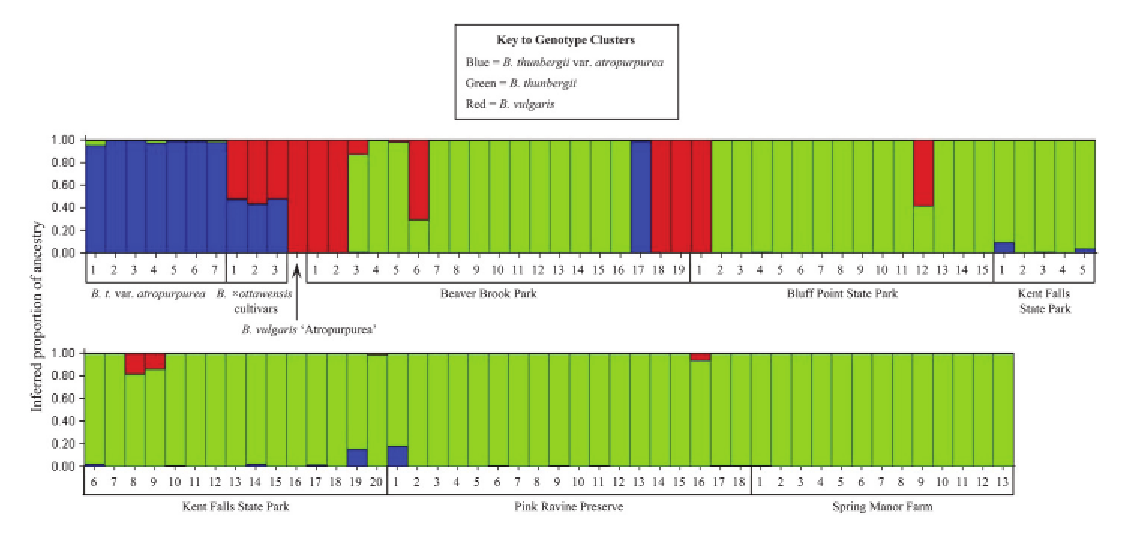
\includegraphics{lubell-structure.eps}}
\caption{Analysis of AFLP data from {\it Berberis
    thunbergii}}
\end{figure}
}

\myslide{
\begin{itemize}

\item Human Genome Diversity Cell Line Panel (HGDP-CEPH)

\item 1056 individuals, 52 geographic populations, 377 autosomal
  microsatellite loci

\end{itemize}

\begin{figure}
\resizebox{\textwidth}{!}{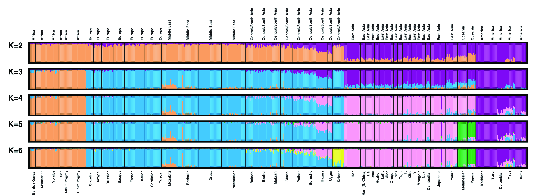
\includegraphics{HGDP-CEPH.eps}}
\end{figure}

}

\myslide{
\begin{itemize}

\item Principal components analysis of genotypes.

\item 3129 Europeans, 500,568 SNP loci

\end{itemize}

\begin{figure}
\begin{center}
\resizebox{0.5\textwidth}{!}{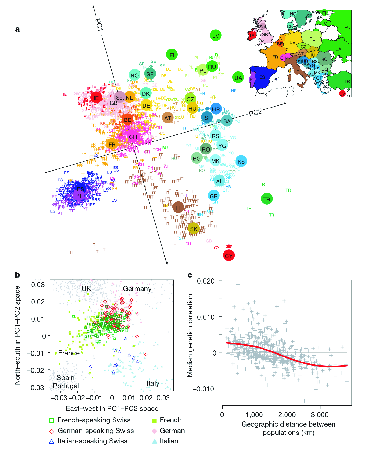
\includegraphics{human-PCA.eps}}
\end{center}
\end{figure}

}

\end{document}

